\documentclass{article}
\usepackage[margin=24mm]{geometry}
\usepackage{tikz}
\title{Full reverse-jet state and computation search}
\date{Created-at: 2026-10-30 09:15 +01:00}
\begin{document}\maketitle
\paragraph{Accepted correction.} The requested object is the complete24-bit
reverse jet, not another six-bit scalar. Pgraph must generate networks before
native gates exist. No complete-circuit candidate list, no fixed active-span
restriction, and no monotone-cost-only admission. Preserve all phase debts and
score in the complete decoder context. User subsequently requested execution on
this machine: Windows compilation/search and the existing local WSL Python
runtime for the supplied Linux kickmix ABI; no new Amaterasu campaign.
\paragraph{Source model.} Author typed quantum/classical/token state versions,
storage identities and read/take/give hyperedge ports for the entire reverse.
Include the factored norm/inverse/scaling route and the direct inverse/product
route, decomposed into actual operators. Choices concern N retention or
recomputation, k retention or norm reconstruction, multiplication algorithms,
and phase cleanup. They are alternative producers of functional states, not
names of complete circuits. Explicit phase-closure tokens constrain schedules.
\paragraph{Ordering and ownership.} Core/Query retain the authored model.
Existing Pgraph MSG/SSG enumerate structures. Quantum admits unique producers,
single destructive consumers and complete reachable goals. Its resource-aware
interpreter searches executable orders with read-before-destroy constraints.
Only selected networks reach the native backend. Afterwards, exact GF(2)
linear-view elimination can replace compute/use/uncompute square copies with
invertible control frames. This elimination concerns linear view constraints,
not a claim that the entire nonlinear decoder is a linear Schur problem.
\paragraph{Native operators.} Reuse reviewed arithmetic primitives, not the
public complete reverse routine: norm, start/finish inverse, products, scaling,
phase correction and erasure. Bind canonical state IDs to ephemeral native
register handles. The executor has no retained/direct whole-circuit mode switch.
It must reject missing/retired state, mismatched dimensions or open phase debt.
The public complete reverse remains an independent comparison oracle.
\paragraph{Files.} Add synthesis/reverse.rs, separate reverse vocabulary/model,
focused Rust tests and native operator executor under the existing Quantum
package. Extend synthesis exports/CLI, HermiteLibrary, quantum\_network.py,
report.py and README. Existing scalar/closed-span search remains a separate
bounded capability and is not called the full search. No Core/Graph/provider
source or dependency change is planned; protected CORE.YAML items=[]
\paragraph{Acceptance.} Source producer edits must change generated networks
before native code is invoked. Reproduce the complete reference reverse's
Q/T and independently verify its value/phase behavior. At least one generated
network must change an N/k lifetime; native logs must show the changed allocation.
Verify self and cross jet pairings, source identity and cleanup. Native measured
costs update candidate ordering/selection; estimates alone cannot promote a
circuit. Only a promising complete-context candidate proceeds to the unchanged
102400-shot local verifier; no Kaggle submission.
\paragraph{Budgets and risks.} Initial structure cap16384 (hard ceiling65536),
at most64 states/64 operations, eight schedule states retained, at most64 native
probes initially. Explicit capped/incomplete statuses; no optimality claim.
Native small probes: one CPU,512MiB process-tree guard,900s per bounded batch.
Windows currently has little free physical memory, so do not start Docker or a
large full verifier without checking resources again. Existing local source,
official data and Python3.13 runtime are present; no repository copies.
ETA90--150min from this plan for implementation, local checks and evidence;
full verification, if justified and resources permit, has a separate guard.
\paragraph{Repository and rollback.} Transformation feat/unversioned c90eb2b,
fresh fetch succeeded/current. Preserve unrelated dirty work and all incumbents.
No commit/push/merge. Roll back only named task edits. Report exact limitations
and archive once after report writers stop. Failure to beat the incumbent is not
permission to present scalar improvements as the requested full optimizer.
\paragraph{Continuation, 2026-10-30 12:22 +01:00.} User explicitly authorizes
offline edits to the existing Graph/Transformation checkouts after failed Gitea
fetches. GitHub fetch succeeded but does not contain the working task branches.
Graph HEAD d006ba5; Transformation c90eb2b; preserve all unrelated dirty work.
Implement generic partial-decision constraints in the existing Pgraph SSG owner:
exclusive producers and unit groups, finite node/output caps, and an optional
nonnegative cost-cover relaxation. Old unconstrained API retains its semantics.
Quantum exports source-bound constraints and admits source-bound structure
receipts, without enumerating first. The existing Pgraph CLI transports receipts;
no dependency repin, local path override or duplicate search engine.
\paragraph{Inner search.} Extend Graph's binary matroid owner with a bounded
input/output lifetime frontier, reusing exact column-basis reconstruction.
For a product emitted now, count remaining input rank before retirement plus
accumulated output rank after insertion. This is an optimistic separate-bank
linear representation, not a general quantum-space theorem or a gate emitter.
Small exhaustive orders certify the heuristic against the declared family;
the actual 99-product source is a functional validation input. Exact rank and
coverage certificates can support bounds only within their stated scope.
\paragraph{Continuation interfaces and files.} Graph: ssg\_dm.rs, cli.rs,
bin/pgraph.rs, tests in ssg\_dm.rs; matroid/binary.rs and mod.rs, existing
matroid\_binary tests and binary\_matroid example; CORE.YAML approval record,
README. Transformation: synthesis/reverse.rs and exports, quantum\_synthesis CLI,
reverse\_state tests, quantum\_network.py, reverse\_state.py authoring support,
test\_reverse\_state.py, existing README/report files. Protected owners
hymeko\_pgraph and hymeko\_graph are explicitly requested by the user; no other
protected capability or dependency changes. Core itself remains unchanged.
\paragraph{Continuation checks and limits.} Preserve all admissible small
structures; verify capped-prefix behavior, invalid-constraint rejection,
relaxation soundness versus full small enumeration, and exact rank coordinates.
The full24 source must reproduce previous valid program identities before gates.
No new native campaign if emitted operators/orders are identical. No runtime
benchmark; structural counters and deterministic correctness only. Existing
memory guards apply to any native tensor export. ETA60--90min for owner APIs,
consumer integration and targeted checks, with the frontier feasibility result
reported even if it proves no saving. Final reports archive when Samba returns.
\paragraph{Three-family continuation, 2026-10-30 14:01 +01:00.}
User authorizes all three mathematical directions: new intermediates, joint
product/phase/cleanup, and alternative arithmetic decompositions in Pgraph.
Offline authorization persists; Gitea TCP2222 is still unavailable. Only the
existing Transformation checkout changes in this phase; Graph APIs are reused.
Before code, define a joint reverse contract: after early replacement of u by
inverse0(u) and v by its scaled result, combine old-u and old-v masks through
$L=\mu+S^T M_v^T\nu$. The residual zero-case phase is
$F(\nu\cdot v+f_z)$. Realize $L\cdot\mathrm{inverse0}(u)$ via a12-bit
coefficient and inverse phase. Two producers compute that coefficient: exact
transposed multiplication, and norm polarization using the field-trace dual
map. Every norm/inverse/flag debt remains explicit.
\paragraph{Cache families and ownership.} Preserve zero, one or two existing
scalar intermediates from the reviewed cached-inverse primitive, through a
strict allocation/erasure adapter, without copying its arithmetic algorithm.
These are norm(u-new)12 and norm(norm(u-new))6. The selected source operations
retain or reconstruct these values, create the joint coefficient, apply inverse
phase, repay measured coefficient phase and close all states. The tensor99 and
105 product alternatives remain; the old source/model remains reproducible.
Add joint\_phase.py in the existing native Quantum package; extend reverse\_state.py,
hermite.py's optional cached norm interface, Rust reverse signatures/model,
quantum\_network.py/model option, quantum\_hermite.py checks, existing tests,
README/report. Add reverse\_joint.hymeko generated by the same author. No rank
solver, Pgraph engine, dependency or public-source copy is introduced.
\paragraph{Checks and limits.} Certify the transposed-mask identity and norm
polarization algebra with independent finite-field operations. Verify cache
relations and the zero case. Every full candidate must pass all three cross
forward pairings, phase and clean-workspace tests, plus actual operator resource
profiles. Source-first generation uses the existing early constraints and source
digests. At most64 states/operators and64 native probes,512MiB/900s per probe;
no automatic full verifier unless complete-context cost improves. ETA60--100min
after this algebraic design for implementation and bounded validation. An honest
negative cost result is retained; no scalar-only result or unchanged permutation
search is substituted for the full24 target. Rollback only these named additions.
\paragraph{Integration finding, 2026-10-30 15:16 +01:00.} The new dependency
family exposed unsupported producer cycles in SSG decision-mapping leaves.
The Quantum admission correctly refused them. Scope expanded to the existing
Graph SSG owner: apply the already-owned forward-feasibility predicate before
materializing leaves. A small raw/unsupported-cycle regression passes; the old
20-structure result is unchanged. This is a correctness repair, not another
Pgraph implementation or a relaxation of the domain checks.
\paragraph{Primer and implementation review, 2026-10-30 20:04 +01:00.}
User requests a mathematical/physical primer, followed by inspection of the
implementation. Deliver a Hungarian standalone primer.tex in this directory,
its PDF and validation receipts under the existing joint-functions report
directory, a README link and an appended section in the existing task report.
Extend this plan's Mermaid view to document the two-stage delivery.
Acceptance: distinguish exact identities, existing implementation, measured
results and research hypotheses; derive the phase/value contract, functional
hyperedges, phase factoring, finite-field norm/trace duality, matroid bounds,
Pgraph relaxation and GF(2) Schur elimination. Map each capability to its actual
owner and specify the missing joint phase search without inventing a second IR.
Check primary references and existing evidence, rerun only the three relevant
existing phase correctness tests, and independently check the small-field
algebraic examples. Compile and inspect the PDF. No production algorithm,
dependency, protected Core item, native campaign or official score changes.
The source tree remains dirty from recorded parallel work; preserve it.
Both origin and GitHub fetches succeeded; HEAD equals origin/feat/unversioned.
ETA25--40min for derivations, source review, rendering and archival. No
performance measurement; bounded small correctness work only. Rollback is
limited to these documentation additions; prior measured reports stay intact.
Main risks: confusing GF(2) with Z8, mistaking rank for nonlinear complexity,
and calling a local phase template the full24 optimizer. Explicitly label all
three boundaries. Reuse existing owners and verification instead of expanding
the eight-variable truth table to24 variables.
\paragraph{Illustrated primer continuation, 2026-10-30 20:25 +01:00.}
User requests more figures in the existing primer. Extend primer.tex with eight
vector illustrations: measurement phase correction, CNOT views, CCZ factoring,
matroid reconstruction, illustrative lifetimes, norm/inverse dependencies,
current versus proposed joint phase, and GF(2) Schur elimination. Caption every
figure and distinguish measured, exact and hypothetical content. Reuse the
existing TikZ renderer and report destinations; no production code or new
algebra is changed. Rebuild the PDF, inspect every figure at readable scale and
check references/layout. Refresh document hashes while retaining the existing
correctness evidence; no test or benchmark rerun is needed for illustrations.
Append the report, update the continuation and archive after rendering stops.
ETA15--25min; no dependency, interface or protected Core changes. Rollback only
this document extension. Both remotes refreshed, origin comparison0/0.
\paragraph{Joint contraction implementation, 2026-10-30 21:00 +01:00.}
User authorizes starting the illustrated primer's implementation, locally.
Deliver an exact scalar phase view of the existing typed bilinear hyperedges,
with Graph-authored parity bases, a direct coefficient-free phase lowering and
source-first Pgraph integration into the full24 reverse. The existing materialized
coefficient route remains a competing producer. This is a bounded first family,
not arbitrary nonlinear synthesis or an RL agent.
\paragraph{Algebra and ownership.} Reuse NativeSynthesis::bilinear\_kernel and
bm\_algebra::kernel\_source. Interpret its certified tensor as the scalar
contraction mask dot multiply(lhs,rhs). Graph's existing binary\_matroid example
supplies basis proposals over the same Core incidence scope; Quantum verifies
source identity, each bank's basis independence and every XOR reconstruction.
Do not add a rank or graph search engine in Python. Emit parity frames and CCZ
through the existing native primitives. The virtual full24 mask remains virtual.
\paragraph{Network alternatives.} Explicitly produce inverse0(norm(u))12,
either using the retained six-bit norm or recomputing the inverse; apply the
scalar phase in raw or certified matroid frames; erase the inverse using the
existing held-flag phase contract. Preserve the zero branch and all old masks.
The inverse register can cost as much as the eliminated coefficient, so count
every allocation, basis operation, inversion and cleanup. No gain is assumed.
\paragraph{Files and interfaces.} Add synthesis/contraction.rs and export its
source-bound phase projection; extend the synthesis CLI, existing synthesis and
reverse tests. Extend joint\_phase.py, reverse\_state.py, HermiteLibrary adapter,
quantum\_hermite.py, quantum\_network.py, existing Python tests, README and report
renderer. Generated phase/reverse sources and receipts live in the existing
reverse-state report tree. Existing Graph owner is reused without edits or repins.
New optional contraction digest and projection arguments must reject absent,
foreign or malformed evidence before native gates. Preserve old source defaults.
\paragraph{Checks and budgets.} Exact small-field tensor, certificate corruption,
phase/input preservation and clean workspace; then bounded full24 self/cross
pairings,6144 shots each, seeds17/31/51. One local CPU,512MiB/900s per native
probe; at most16 new full24 probes and no long run before a passing smoke.
Old64-state/operator,16384-structure and beam8 caps remain explicit. Existing
receipts are reused when source/order is unchanged. No new full official check
unless the complete-context cost improves; no submission. Report negative
results honestly. ETA60--90min for owner extension, tests and bounded execution.
Source is dirty from prior/unrelated work; preserve it. Both remotes refreshed,
origin comparison0/0. No Core items, dependencies, publication or other-host
compute changes. Rollback only this continuation's named source additions.
\paragraph{Lifetime refinement, 2026-10-30 21:29 +01:00.}
The first checked scalar route is418T/Q883. Its phase-time headroom permits a
candidate12-qubit output-mask basis instead of recomputing84 mask parities.
Add a bank mode using the same Graph witness; all three banks then participate
physically. It computes/erases12 basis forms per half and reconstructs requested
parities in place. Keep at most two modes in an authored source to preserve the
128-program admission guard. Test the small native bank before a full24 probe.
No Toffoli reduction is assumed; compare actual native instructions and global
peak. Complete-projection fingerprints now bind frame choice as well as tensor.
\begin{center}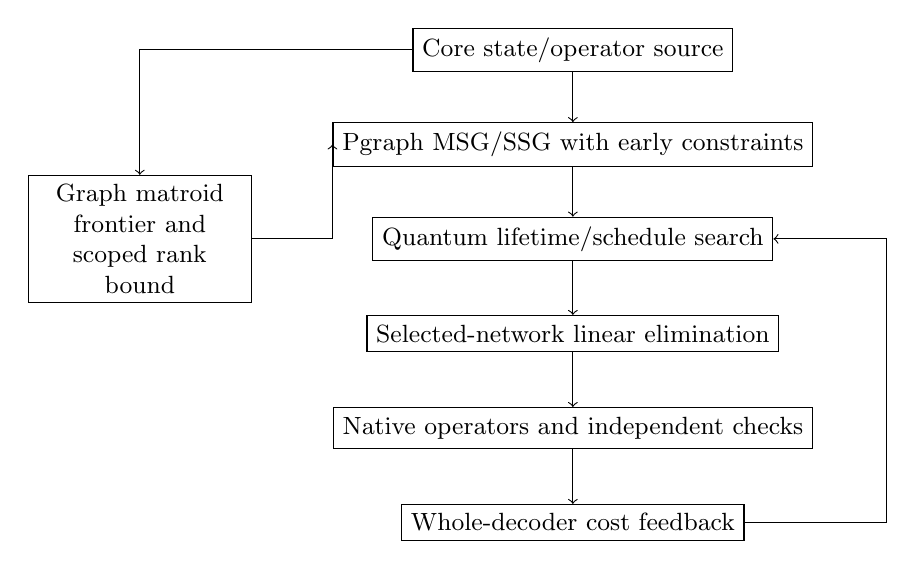
\begin{tikzpicture}[every node/.style={draw,align=center,font=\small},node distance=12mm]
\node(a){Core state/operator source};
\node(b)[below of=a]{Pgraph MSG/SSG with early constraints};
\node(c)[below of=b]{Quantum lifetime/schedule search};
\node(d)[below of=c]{Selected-network linear elimination};
\node(e)[below of=d]{Native operators and independent checks};
\node(f)[below of=e]{Whole-decoder cost feedback};
\draw[->](a)--(b);\draw[->](b)--(c);\draw[->](c)--(d);\draw[->](d)--(e);\draw[->](e)--(f);
\draw[->](f.east)--++(18mm,0)|-(c.east);
\node(g)[left of=c,xshift=-43mm,text width=26mm]{Graph matroid\\frontier and\\scoped rank bound};
\draw[->](a.west)-|(g.north);\draw[->](g.east)-|(b.west);
\end{tikzpicture}
\end{center}
\end{document}
